\section{Descripción de las Etapas de Desarrollo}
En esta sección, se describen las principales etapas del desarrollo del proyecto, 
desde la planificación inicial hasta el despliegue final. Cada etapa jugó un papel 
crucial en la evolución del proyecto, permitiendo una implementación organizada y eficiente de la plataforma OTT.

\subsection{Fase de Análisis y Planificación}
\subsubsection{Recolección de Requisitos}
En esta etapa, se realizó un análisis exhaustivo para identificar los requisitos 
funcionales y no funcionales del proyecto. Esto incluyó reuniones con los clientes
para entender las expectativas y necesidades de cada uno, así como un análisis de mercado para
asegurar que las plataformas cumplieran con los estándares actuales. 

\subsection{Fase de Diseño}
\subsubsection{Diseño de Arquitectura}
Durante esta etapa, se definió la arquitectura general de la plataforma  OTT con sus componentes. Se utilizó 
una arquitectura basada en microservicios para garantizar la escalabilidad y flexibilidad del 
sistema e integración con los servicios existentes en la empresa. También se diseñó la estructura de 
comunicación entre los componentes y se eligieron las tecnologías más adecuadas para cada parte del sistema.

Se estudiarón los conjuntos de datos y las APIs necesarias para creación de la plataforma de análisis de datos.

\subsubsection{Diseño de la Interfaz de Usuario}
Se comenzó a trabajar sobre una interfaz básica para la plataforma OTT que permitiera el desarrollo de las funcionalidades
principales de la plataforma y poco a poco se fue refinando y mejorando en función de las peticiones
de los clientes y las pruebas de usabilidad realizadas. A través de reuniones con los clientes y 
analizando sus peticiones y prototipos, se fueron contruyendo los diseños de manera conjunta hasta
llegar a un diseño final que satisfaciera las necesidades de los usuarios.

Se diseño la interfaz de usuario para la plataforma de análisis de datos, con el objetivo de que los usuarios
pudieran visualizar y analizar los datos de manera sencilla y efectiva sin necesidad de conocimientos técnicos.

\subsection{Fase de Desarrollo}
\subsubsection{Implementación de Funcionalidades}
Esta fase fue el núcleo del proyecto, donde se desarrollaron las funcionalidades clave de la 
plataforma OTT. Cada funcionalidad se implementó de manera incremental, siguiendo un ciclo 
ágil de análisis, diseño, codificación y pruebas. Se utilizaron tecnologías web como JavaScript, 
HTML y CSS para asegurar la compatibilidad multiplataforma.

Para la plataforma de análisis de datos, se implementaron las funcionalidades necesarias para
la carga, procesamiento y visualización de los datos, así como de análisis y generación de informes.

\subsubsection{Optimización y Refactorización}
A medida que se añadían nuevas funcionalidades, el código se refactorizaba y optimizaba para 
mejorar el rendimiento y la mantenibilidad. Este proceso incluyó la simplificación de la lógica 
de negocio, la mejora de la estructura del código, y la optimización de la carga y la respuesta de la aplicación.

\subsection{Fase de Pruebas}
\subsubsection{Pruebas Unitarias y de Integración}
Se realizaron pruebas unitarias para cada componente, asegurando que las funciones individuales 
funcionaran correctamente. Luego, se realizaron pruebas de integración para verificar que los 
componentes interactuaran de manera efectiva y sin conflictos.

\subsubsection{Pruebas de Compatibilidad}
Se llevaron a cabo pruebas exhaustivas en diferentes dispositivos y sistemas operativos 
(web, Tizen, WebOS, Android TV) para asegurar que la aplicación funcionara correctamente 
en todos los entornos previstos. Esto incluyó pruebas de rendimiento para garantizar que 
la aplicación se ejecutara sin problemas en dispositivos con capacidades de hardware limitadas.


\subsection{Conclusión}	  
Estas etapas se llevaron a cabo de manera iterativa y colaborativa, con reuniones periódicas
con los clientes para validar el progreso y ajustar las prioridades según fuera necesario.
Así para cada funcionalidad nueva se realizaba un ciclo de análisis, diseño, implementación y pruebas
para asegurar que la funcionalidad cumpliera con los requisitos y expectativas del cliente.


\section{Diagrama de Gantt}
El diagrama de Gantt de la Figura \ref{fig:gantt_chart} muestra la planificación de las etapas del proyecto, 
desde el análisis de viabilidad hasta la entrega final. Cada proyecto se distingue por un color diferente, y 
cada etapa se representa con un tono distinto para facilitar la diferenciación entre las fases.

\begin{figure}[H]
  \centering
  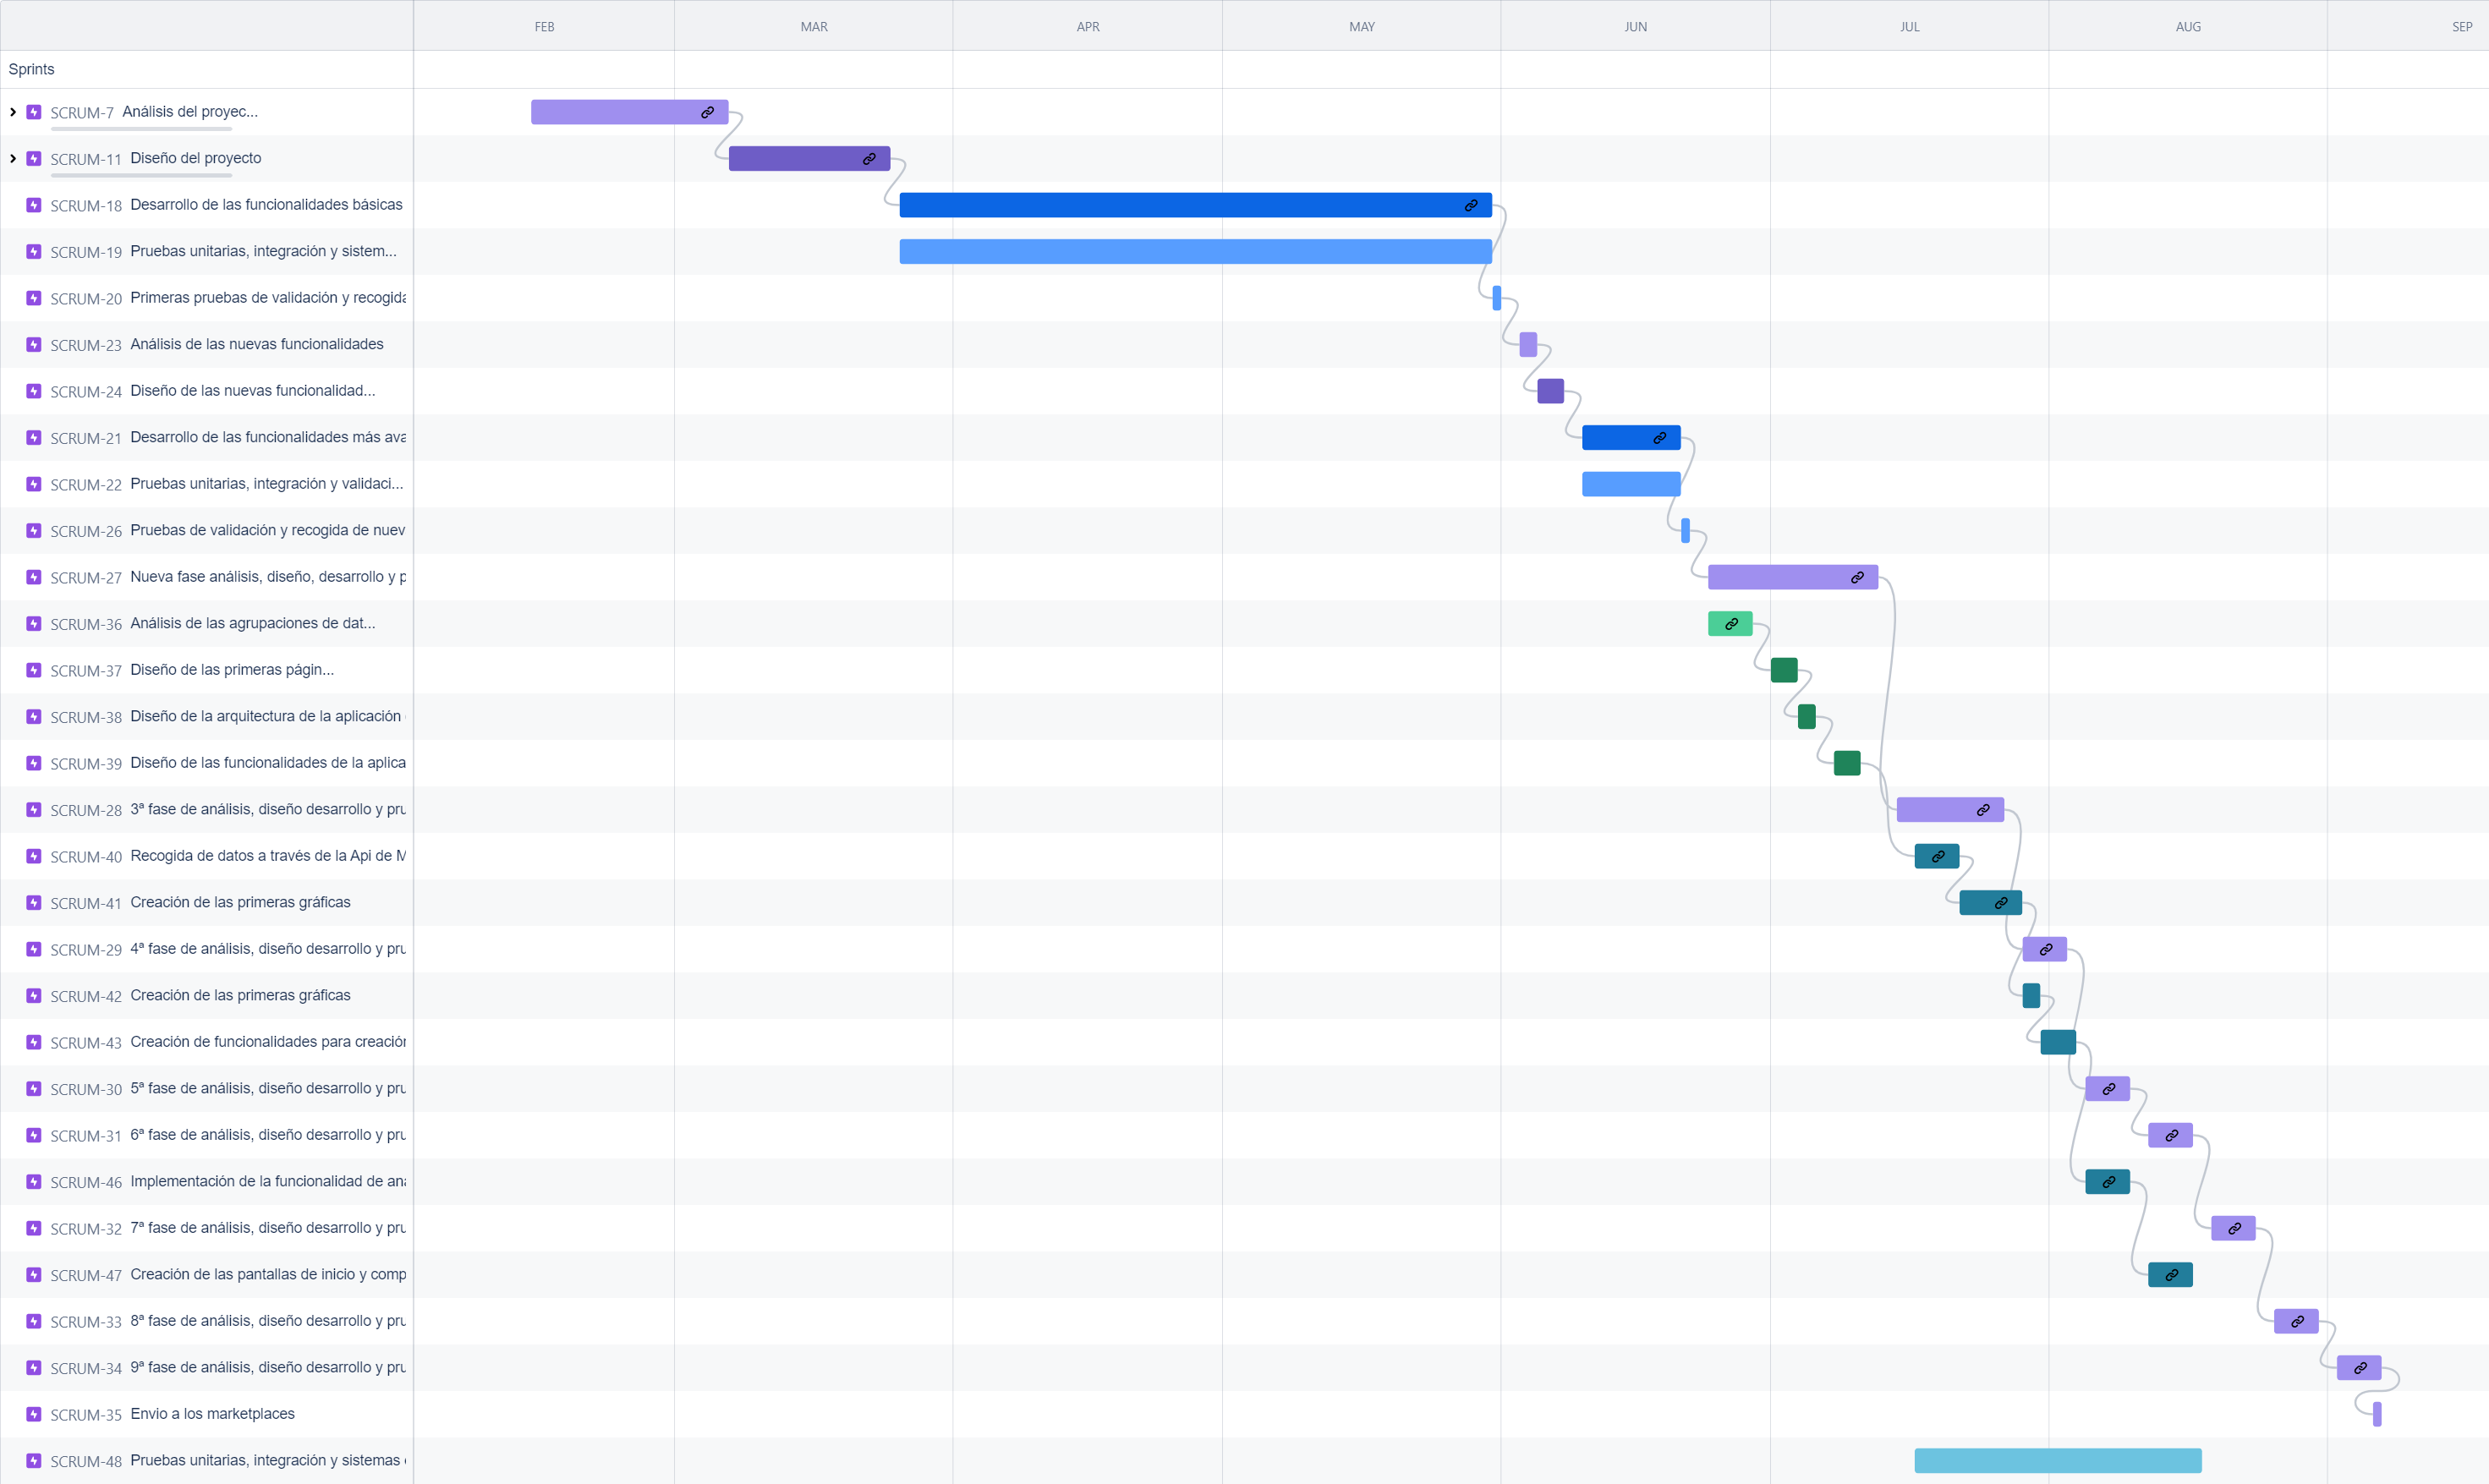
\includegraphics[width=0.9\textwidth]{imaxes/gantt_chart}
  \caption{Diagrama de Gantt del Proyecto}
  \label{fig:gantt_chart}
\end{figure}

Como se puede apreciar en la Figura \ref{fig:gantt_chart}, el proyecto se dividió en varias etapas, cada una 
de ellas con tareas y subetapas asignadas. La planificación de cada etapa se estableció para un tiempo determinado, 
y se llevaron a cabo reuniones periódicas para evaluar el progreso y realizar los ajustes necesarios en la planificación.

Cada etapa está compuesta por:
\begin{itemize}
    \item Una fase de \textbf{análisis}, donde se evaluaban los requisitos y las posibles soluciones.
    \item Una fase de \textbf{diseño}, en la que se definían los detalles técnicos y de la interfaz.
    \item Una fase de \textbf{desarrollo}, que involucraba la implementación de las funcionalidades y optimización de las mismas.
    \item Una fase de \textbf{pruebas}, que incluía la validación de la funcionalidad y la realización de ajustes según fuera necesario.
\end{itemize}

Se realizaron reuniones periódicas con los clientes para validar el progreso y ajustar las prioridades conforme avanzaba el proyecto.

\paragraph{Explicación detallada del diagrama de Gantt:}

\begin{enumerate}
    \item \textbf{Análisis del Proyecto:} La primera etapa incluyó el análisis de viabilidad y la planificación de las fases iniciales. 
    Esto permitió definir claramente los objetivos y establecer un calendario preliminar para el resto del desarrollo.
   
    \item \textbf{Diseño del Proyecto:} Se desarrolló la estructura básica y se realizaron los primeros bocetos de la 
    interfaz de usuario y la arquitectura de microservicios. Este paso fue fundamental para asegurar que el diseño fuera 
    escalable y adaptable a las diferentes plataformas.

    \item \textbf{Desarrollo de Funcionalidades Básicas:} Una vez que se establecieron las bases del diseño, comenzó el desarrollo 
    de las funcionalidades clave de la plataforma OTT y la plataforma de análisis de datos.

    \item \textbf{Pruebas Unitarias e Integración:} Durante todo el proceso, las funcionalidades fueron sometidas a pruebas para 
    asegurar que todas las partes del sistema funcionaran correctamente antes de proceder con nuevas implementaciones.

    \item \textbf{Validaciones y Mejoras Continuas:} Se realizó una validación constante de las funcionalidades mediante pruebas 
    de usuario y reuniones con los clientes. También se ajustaron las funcionalidades según la retroalimentación recibida.

    \item \textbf{Despliegue Final y Entrega:} En la última etapa, se realizaron pruebas finales en los marketplaces y se preparó 
    la aplicación para su lanzamiento, asegurando que cumpliera con los requisitos de las distintas plataformas y que estuviera 
    lista para ser publicada.
\end{enumerate}

Como se muestra en el diagrama de Gantt, las fases de diseño, desarrollo y pruebas están interconectadas, con dependencias claras 
que marcan cómo cada tarea debía completarse antes de avanzar a la siguiente. Esto permitió un seguimiento detallado del progreso 
y facilitó la identificación de posibles retrasos o áreas que requerían ajustes.

